\documentclass[Main.tex]{subfiles}
\begin{document}
	
	\begin{description}
		\item[residuals.lme] 
		The residuals at level $i$ are obtained by subtracting the fitted levels at that level from the response
		vector (and dividing by the estimated within-group standard error, if \texttt{type="pearson")}. The fitted
		values at level $i$ are obtained by adding together the population fitted values (based only on the
		fixed effects estimates) and the estimated contributions of the random effects to the fitted values at
		grouping levels less or equal to $i$.
	\end{description}
	
	
	\chapter{Residual Analysis}
	A residual is the difference between an observed quantity and its estimated or predicted value. In LME models, there are two types of residuals, marginal residuals and conditional residuals. A marginal residual is the difference between the observed data and the estimated marginal mean. A conditional residual is the difference between the observed data and the predicted value of the observation. In a model without random effects, both sets of residuals coincide.
	
	\section{Residual diagnostics} %1.3
	\subsection{Introduction to Residual Analysis}
	%A residual is the difference between an observed quantity and its estimated or predicted value. 
	Residual analysis is a widely used model validation technique. A residual is simply the difference between an observed value and the corresponding fitted value, as predicted by the model. The rationale is that, if the model is properly fitted to the model, then the residuals would approximate the random errors that one should expect; if the residuals behave randomly, with no discernible trend. If some sort of non-random trend is evident in the model, then the model can be considered to be poorly fitted.
	
	For classical linear models, residual diagnostics are typically implemented as a plot of the observed residuals and the predicted values. A visual inspection for the presence of trends inform the analyst on the validity of distributional assumptions, and to detect outliers and influential observations. Statistical software environments, such as the \texttt{R} programming language, provides a suite of tests and graphical procedures for appraising a fitted linear model, with several 
	of these procedures analysing the model residuals.
	
	However, for LME models the matter of residual is more complex, both from a theoretical point of view and from the practical matter of implementing a comprehensive analysis using statistical software. As the LME model can be tailored to the needs of the particular research question, the rationale behind the model appraisal must follow accordingly.
	
	
	%===================================================================================================%
	\subsection{Residuals in the Blood Data Example}
	The fitted model used in the Blood data example, \texttt{JS.roy1}, was fitted using the \texttt{lme()} function from the nlme package, and as such, is stored as an \texttt{lme} object. The \texttt{residual} functions extracts residuals of a fitted LME model, depending on the type of residual required.
	
	For an lme object, the residuals at level $i$ are obtained by subtracting the fitted levels at that level from the response vector (and dividing by the estimated within-group standard error, if \texttt{type="pearson"}).The Pearson residual is the raw residual divided by the square root of the variance function (here, the Within-group standard error for both methods, 6.11 and 9.11 respectively). The fitted values at level $i$ are obtained by adding together the population fitted values (based only on the fixed effects estimates) and the estimated contributions of the random effects to the fitted values at grouping levels less or equal to $i$.
	
	\begin{description}
		\item["\texttt{response}"]: the “raw” residuals (\textit{observed - fitted}) are used. This is the default option.
		\item["\texttt{pearson}"]: the standardized residuals (raw residuals divided by the corresponding standard errors) are used; 
		\item["\texttt{normalized}"]: the normalized residuals (standardized residuals pre-multiplied by the inverse square-root factor of the estimated error correlation matrix) are used.
	\end{description}
	
	\begin{framed}
		\begin{verbatim}
		data.frame( response = resid(JS.roy1, type = "response"), 
		pearson  = resid(JS.roy1, type = "pearson"), 
		normalized = resid(JS.roy1, type = "normalized") )
		\end{verbatim}
	\end{framed}
	
	\begin{verbatim}
	response      pearson    normalized
	1    -4.65805902 -0.761587227 -0.7615872269
	2    -0.88701342 -0.145025661  0.0776238081
	3    -5.16580898 -0.844603753 -0.8446037530
	4     2.29041830  0.374480726  0.6450898404
	5     7.87508366  1.287567009  1.2875670086
	6    -6.57048659 -1.074266908 -1.5090772378
	...........................................
	\end{verbatim}
	For the $J$ observations, the variance is 6.116252 whereas for the $S$ observations, the denominator is 9.118144. (with the expected ratio of  1.490806)
	
	
	\begin{framed}
		\begin{verbatim}
		> pearson %>%
		+   as.numeric %>% 
		+   matrix(nrow=85) %>%
		+   round(4) 
		[,1]    [,2]    [,3]    [,4]    [,5]    [,6]
		[1,] -0.7616  0.2194  0.3829 -0.2983  0.3597 -0.0790
		[2,] -0.1450  0.1820 -0.1450 -0.5014  0.1567  0.2663
		[3,] -0.8446  0.4634  0.1364 -0.1630 -0.2727  0.1660
		[4,]  0.3745 -0.2795 -0.2795 -0.2658 -0.2658  0.6115
		[5,]  1.2876 -0.6744 -0.6744  0.8935 -0.0935 -0.8612
		[6,] -1.0743  1.8687 -0.7473 -0.0383  0.2908 -0.3673
		...........................................
		
		\end{verbatim}
	\end{framed}
	
	We can plot the residuals against the fitted values, to assess the assumption of constant variance. 
	\begin{framed}
		\begin{verbatim}
		# standardized residuals versus fitted values 
		plot(JS.roy1, resid(., type = "pearson") ~ fitted(.) , 
		abline = 0, id = 0.05)
		\end{verbatim}
	\end{framed}
	\begin{figure}[h!]
		\centering
		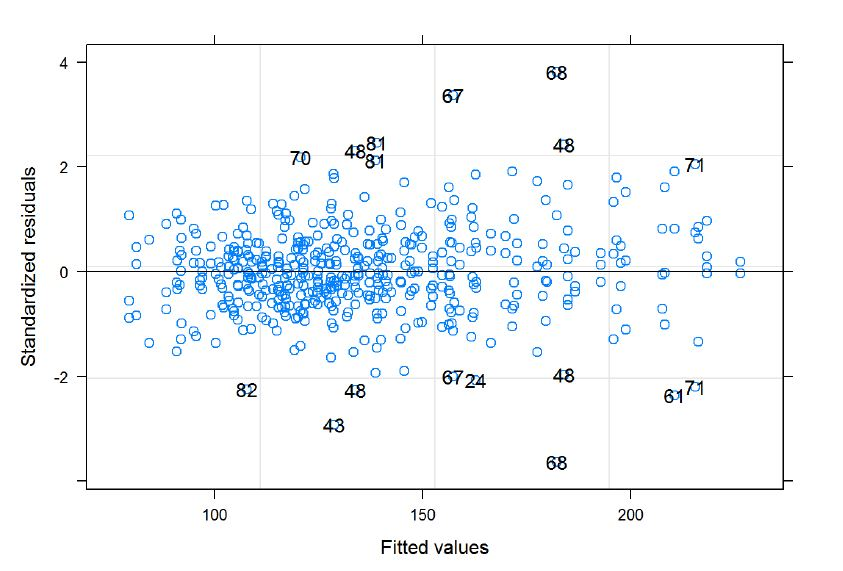
\includegraphics[width=0.9\linewidth]{images/Residuals-JS-Roy}
		\caption{}
		\label{fig:Residuals-JS-Roy}
	\end{figure}
	
	%===================================================================================================%
	\subsection{Normality of Residuals in the Blood Data Example}
	LME models assume that the residuals of the model are normally distributed.  The residuals can be divided according to groups according to the method of measurement. In the following examples, we seperately assess normality the \textit{J} method residuals (the first 255 residuals) and \textit{S} method residuals (the remaining 255). Importantly the residuals from the \textit{J} method are normally distributed, but there is non-normality of the residuals according to the \textit{S} method.
	\begin{framed}
		\begin{verbatim}
		> shapiro.test(resid(JS.roy1)[1:255])
		
		Shapiro-Wilk normality test
		
		data:  resid(JS.roy1)[1:255]
		W = 0.9931, p-value = 0.2852
		\end{verbatim}
	\end{framed}
	
	\begin{framed}
		\begin{verbatim}
		> shapiro.test(resid(JS.roy1)[256:510])
		
		Shapiro-Wilk normality test
		
		data:  resid(JS.roy1)[256:510]
		W = 0.9395, p-value = 9.503e-09
		\end{verbatim}
	\end{framed}
	\begin{figure}[h!]
		\centering
		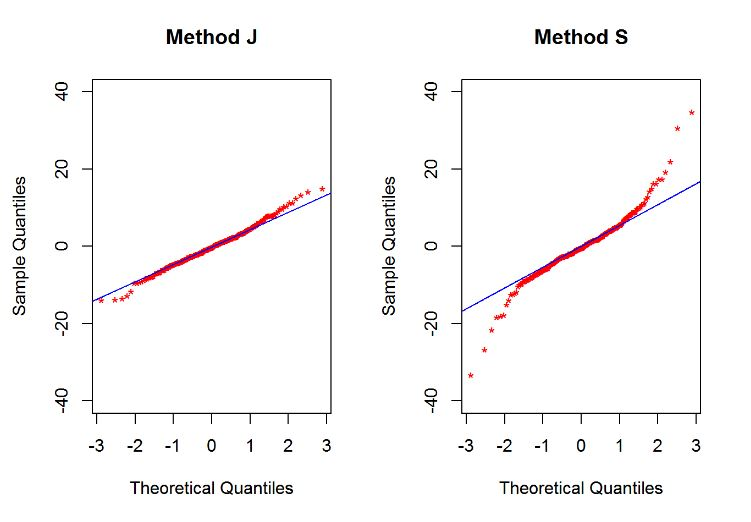
\includegraphics[width=0.9\linewidth]{images/Resid-newplot2}
		\caption{}
		\label{fig:Resid-newplot2}
	\end{figure}
	
	
	
	\subsection{Residual Plots}
	A residual plot is a graph that shows the residuals on the vertical axis and the independent variable on the horizontal axis. If the points in a residual plot are randomly dispersed around the horizontal axis, a linear regression model is appropriate for the data; otherwise, a non-linear model is more appropriate.
	
	\begin{framed}
		\begin{verbatim}
		par(mfrow=c(1,2))
		qqnorm((resid(JS.roy1)[1:255]),
		pch="*",col="red",
		ylim=c(-40,40),
		main="Method J")
		qqline(resid(JS.roy1)[1:255],col="blue")
		qqnorm((resid(JS.roy1)[256:510]),
		pch="*",col="red",
		ylim=c(-40,40),
		main="Method S")
		qqline(resid(JS.roy1)[256:510],col="blue")
		par(mfrow=c(1,1))
		\end{verbatim}	
	\end{framed}
	
	
	\begin{figure}[h!]
		\centering
		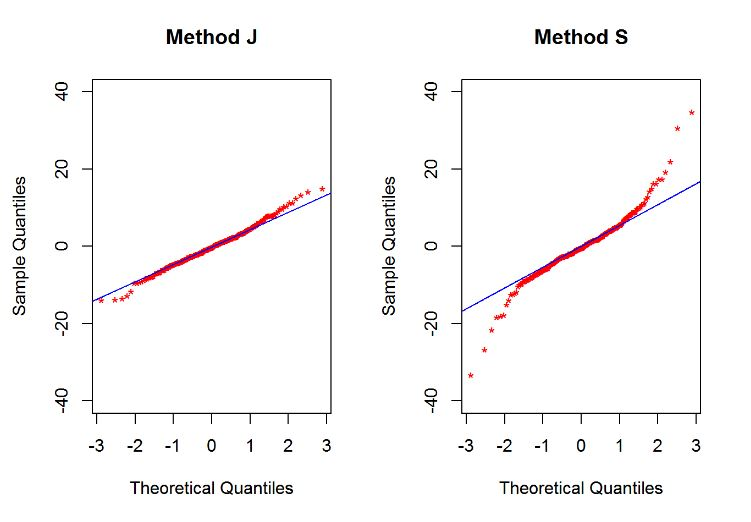
\includegraphics[width=1.1\linewidth]{images/Resid-newplot2}
		\caption{}
		\label{fig:Resid-newplot2}
	\end{figure}
	
	
	\begin{figure}[h!]
		\centering
		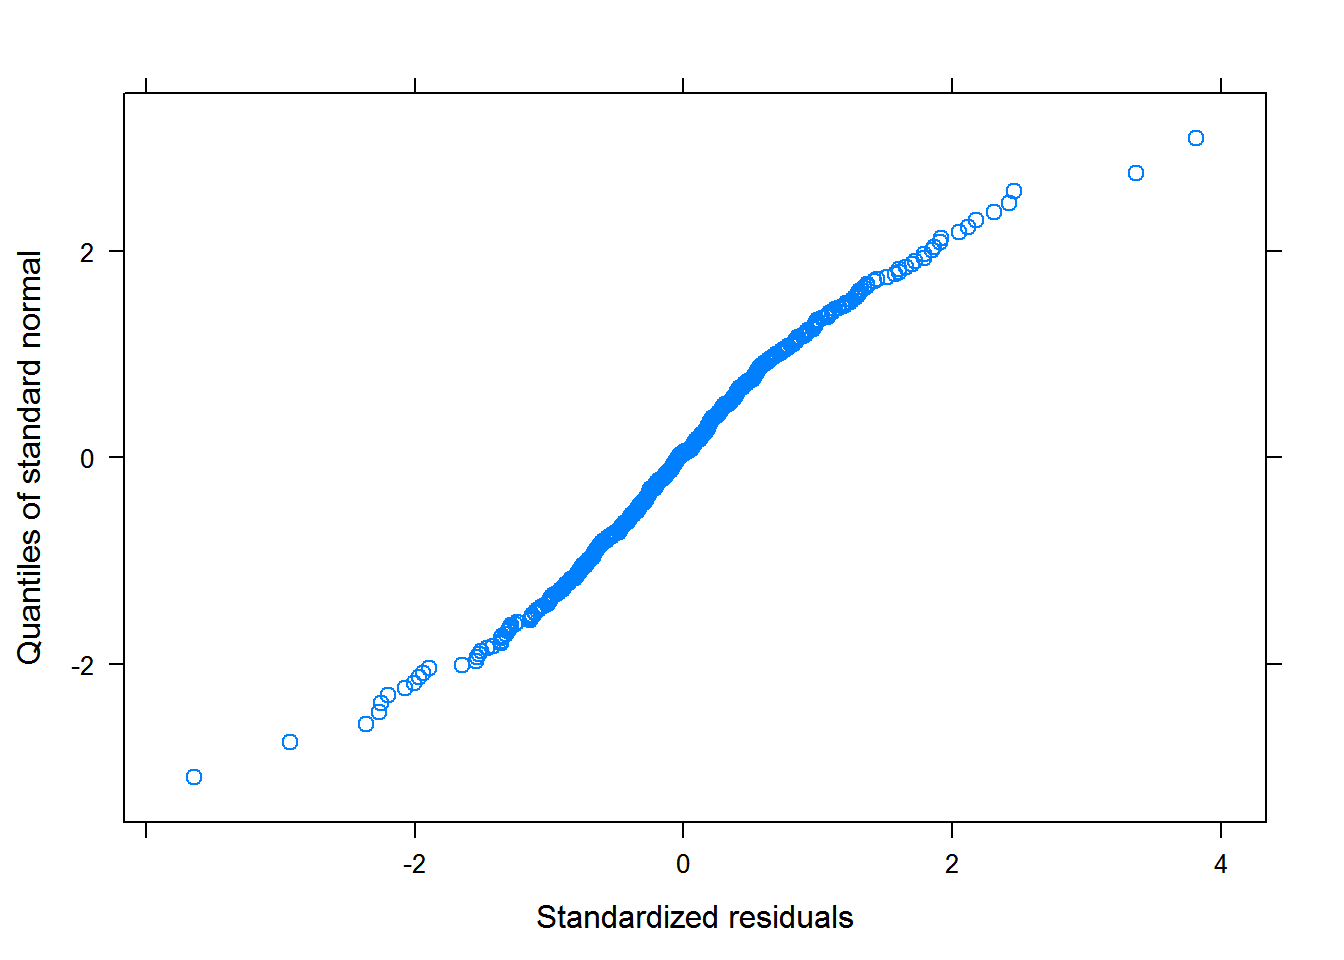
\includegraphics[width=0.9\linewidth]{images/ResidPlot3}
		\label{fig:ResidPlot3}
	\end{figure}
	
	This code will allow you to make QQ plots for each level of the random effects.  LME models assume that not only the within-cluster residuals are normally distributed, but that each level of the random effects are as well. Depending on the model, you can vary the level from 0, 1, 2 and so on
	\begin{framed}
		\begin{verbatim}
		qqnorm(JS.roy1, ~ranef(.))
		
		# 	qqnorm(JS.roy1, ~ranef(.,levels=1)
		\end{verbatim}
	\end{framed}
	\begin{figure}[h!]
		\centering
		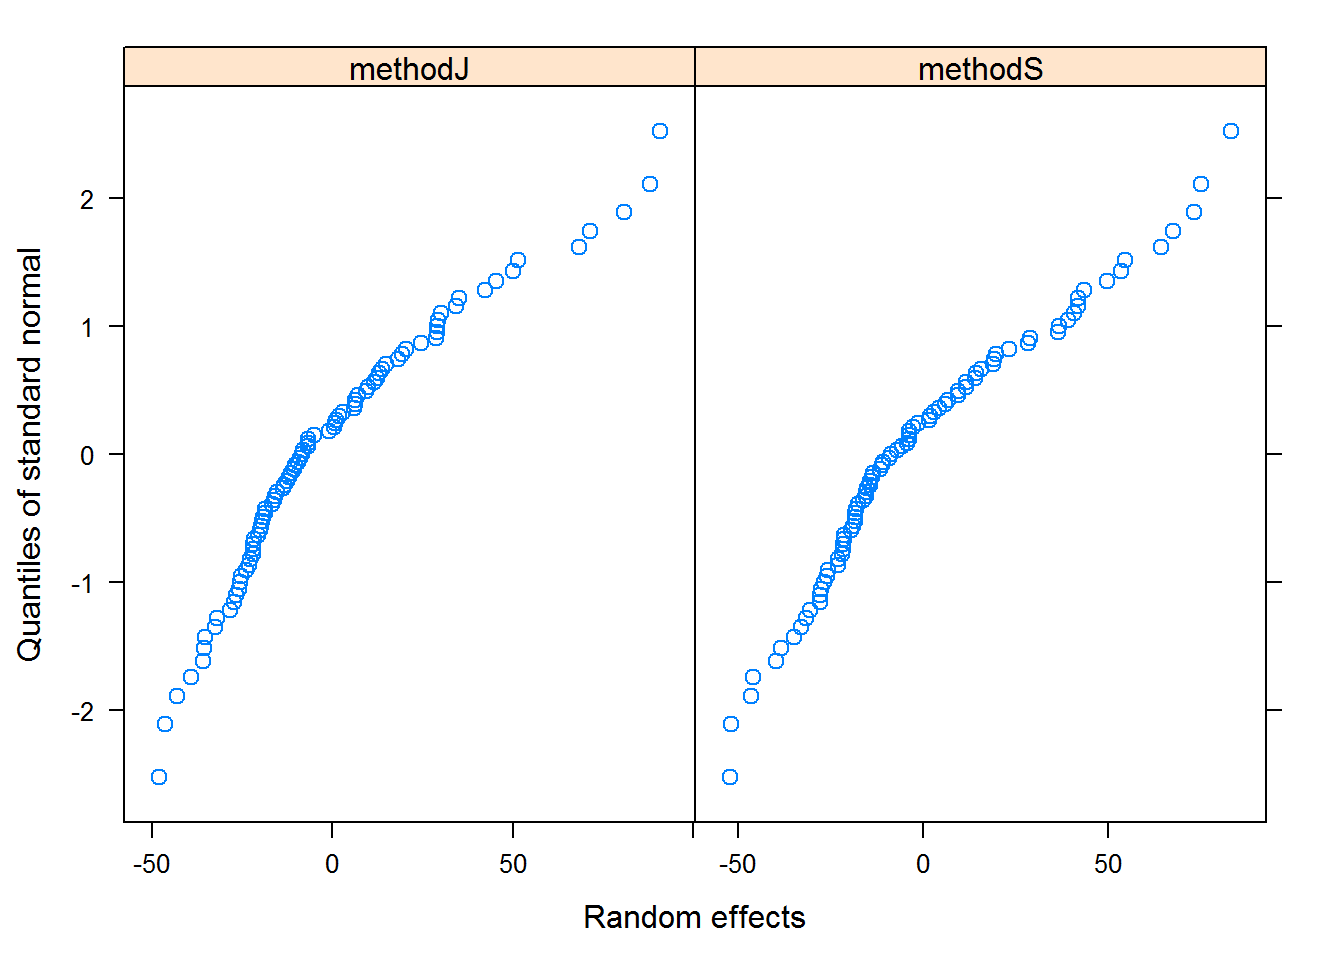
\includegraphics[width=0.9\linewidth]{images/ResidPlot2}
		\caption{}
		\label{fig:ResidPlot2}
	\end{figure}
	
\end{document}